\chapter{Theoretical Motivation} \label{chap-theory}

DGLAP
Higgs related to top
interaction lagrangian with effective operators
electric dipole moment and a top quark with 4/3 charge
anomolous couplings
talk about top quarks - different chapter maybe?

hard-scattering pp collisions
\begin{equation}
\sigma(pp \to X) = \int^1_0dx_1 \int^1_0dx_2 \sum_{a,b} f_a(x_1, \mu_F^2) f_b(x_2, \mu_F^2) \hat{\sigma}_{ab \to X}(Q^2, \mu_F^2)
\end{equation}

\section{The Standard Model of Particle Physics} \label{sec-StandardModel}

\begin{equation}
SU(3)_C \times SU(2)_L \times U(1)_Y
\end{equation}

\begin{equation}
\lumi = \bar{\psi}(i \gamma^{\mu}\delta_{\mu}-m)\psi
\end{equation}

\begin{equation}
\psi \to \psi'= e^{i \theta}\psi, \quad \bar{\psi} \to \bar{\psi}' = e^{- i \thehta}\bar{\psi}
\end{equation}

\subsection{The Electroweak Theory} \label{subsec-ElectroweakTheory}

\begin{equation}
\lumi_{EWK} = \bar{\psi}_L \gamma^{\mu} \left(i \idelta_{\mu} - g\textbf{T} \cdot \textbf{W}_{\mu} - \frac{g'}{2} Y B_{\mu}\right)\psi_L + \bar{\psi}_R \gamma^{\mu}\left(i \idelta_{\mu} - \frac{g'}{2} Y B_{\mu}\right)\psi_R - \frac{1}{4}\textbf{W}_{\mu \nu}\textbf{W}^{\mu \nu} - \frac{1}{4} B_{\mu \nu} B^{\mu \nu} 
\end{equation}

\subsection{Quantum Chromodynamics} \label{subsec-QuantumChromodynamics}

\begin{equation}
\lumi_{QCD} = \bar{q}\left(\gamma^{mu}\delta_{\mu} - m \right) q + g_s \left( \bar{q}\gamma^{\mu}T_a q \right) G^a_{\mu} - \frac{1}{4}G^a_{\mu \nu}G^{\mu \nu}_a
\end{equation}


\begin{equation} \label{equ-ckm}
\begin{pmatrix}
d' \\
s' \\
b' 
\end{pmatrix}
=
\begin{pmatrix}
V_{ud} & V_{us} & V_{ub} \\
V_{cd} & V_{cs} & V_{cb} \\
V_{td} & V_{ts} & V_{tb} 
\end{pmatrix}
\begin{pmatrix}
d \\
s \\
b 
\end{pmatrix}
\end{equation}

\begin{equation} \label{equ-ckm}
V_{CKM}
=
\begin{pmatrix}
0.97425 \pm 0.00022 & 0.2253 \pm 0.0008 & 0.00413 \pm 0.00049 \\
0.225 \pm 0.008 & 0.986 \pm 0.016 & 0.0411 \pm 0.0013 \\
0.0084 \pm 0.0006 & 0.040 \pm 0.0027 & 1.021 \pm 0.032} 
\end{pmatrix}
\end{equation}



\subsection{Electroweak Symmetry Breaking} \label{subsec-ElectroweakSymmetryBreaking}

\begin{equation}
\phi = 
\begin{pmatrix}
\phi^+ \\
\phi^0
\end{pmatrix}{
= \frac{1}{\sqrt{2}}
\begin{pmatrix}
\phi_1 + i \phi_2 \\
\phi_3 + i\phi_4
\end{pmatrix}
\end{equation}

\begin{equation}
\lumi_{Higgs} = (D_{\mu}\phi)^{\dagger}(D^{\mu}\phi) - V(\phi)
\end{equation}

\begin{equation}
V(\phi) = -\mu^2(\phi^{\dagger}\phi) + \lambda(\phi^{\dagger}\phi)^2
\end{equation}

\begin{figure}
\begin{center}
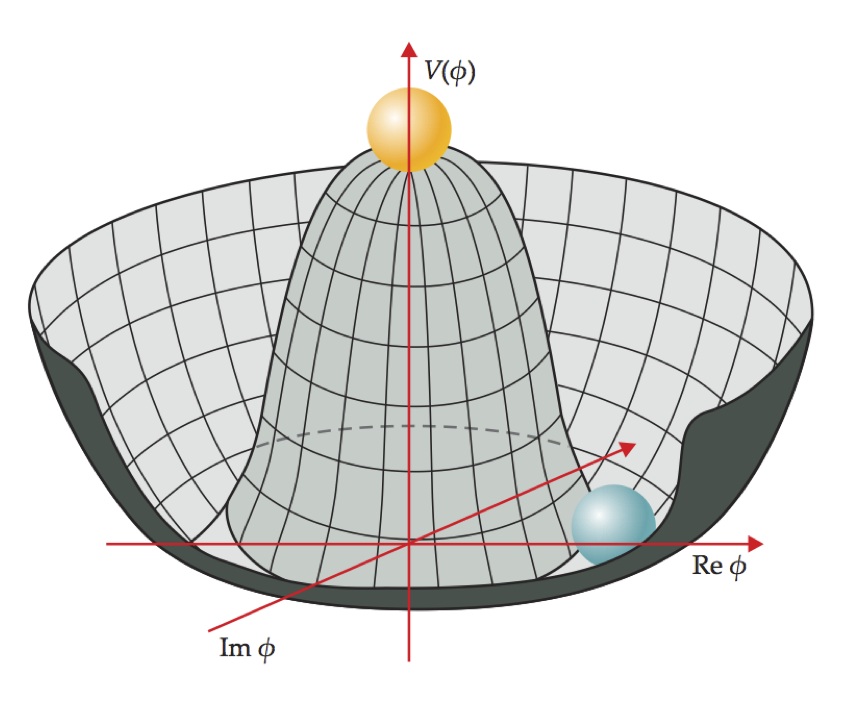
\includegraphics[width=0.7\textwidth]{Figures/MexicanHatPotential.png}
\caption{The ``Mexican Hat Potential" describing the vacuum expectation value of the Higgs in the real and imaginary planes, such that the minima lies below zero.}
\end{center}
\end{figure}

\begin{equation}
\braket{0|\phi|0} = \frac{1}{\sqrt{2}}
\begin{pmatrix}
0 \\
v
\end{pmatrix}
\end{equation}

\begin{equation}
\phi = \frac{1}{\sqrt{2}}
\begin{pmatrix}
0 \\
v + H
\end{pmatrix}
\end{equation}

\begin{equation}
\lumi_{Higgs} = \frac{1}{2}(\delta_{\mu}H)(\delta^{\mu}H) + \frac{1}{4}g^2 (H^2 + 2vH + v^2) W^+_{\mu} W^{-\mu} + \frac{1}{8} (g^2 + g'^2) (H^2 + 2vH + v^2) Z_{\mu} Z^{\mu} - \mu^2 H^2 - \frac{\lambda}{4} (H^4 + 4vH^3)
\end{equation}

\begin{figure}
\begin{center}
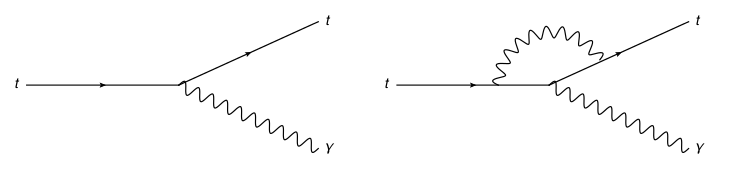
\includegraphics[width=\textwidth]{Figures/TopPhotonVertex.png}
\caption{Top-photon vertex. Left: Leading Order (LO). Right: One-Loop correction (NLO).}
\end{center}
\end{figure}

\begin{equation} \label{eqn-interactionlagrangian}
\lumi_{\gamma t\bar{t}} = -eQ_t\bar{t}\gamma^{\mu}tA_{\mu} - e\bar{t}\frac{i\sigma^{\mu\nu}q_{\nu}}{m_t}(d^{\gamma}_V+id^{\gamma}_A\gamma^5)tA_{\mu}
\end{equation}

\begin{equation}
\lumi^{eff.} = \Sum \frac{C_x}{\Lambda_x}O_x + ... ,
\end{equation}

\begin{align}\label{eqn-smparameterisations}
\delta d^{\gamma}_V = \frac{\sqrt{2}}{e}\text{Re}[c_WC^{33}_{uB\phi} + s_WC^{33}_{uW}]\frac{vm_t}{\Lamdba^2} \\
\delta d^{\gamma}_A = \frac{\sqrt{2}}{e}\text{Im}[c_WC^{33}_{uB\phi} + s_WC^{33}_{uW}]\frac{vm_t}{\Lamdba^2}
\end{align}

\begin{figure}
\begin{center}
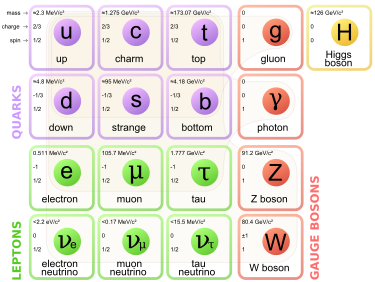
\includegraphics[width=0.8\textwidth]{Figures/StandardModel.png}
\caption{The Standard Model of particle physics.}
\end{center}
\end{figure}

\section{The Top Quark} \label{sec-TheTopQuark}

\begin{table} \label{tab:mumu_cutflow}
\begin{center}
\begin{tabular}{lccc}
\hline
\hline
\textbf{$\sqrt{s}$} & \textbf{$\sigma_{tot.}$} & \textbf{scales [pb]} & \textbf{pdf [pb]} \\
\hline
Tevatron 1.9 TeV & 7.164 & & \\
LHC TeV & 172.0 & $^4.4_5.8$ &  \\ 
LHC 8 TeV & 245.8 & & \\
LHC 14 TeV & 953.6 & & \\
\hline
\hline
\end{tabular}
\caption{\cite{Czakon:2013goa}}
\end{center}
\end{table}

\begin{figure} \label{fig-ttbarProductionLHC}
\begin{center}
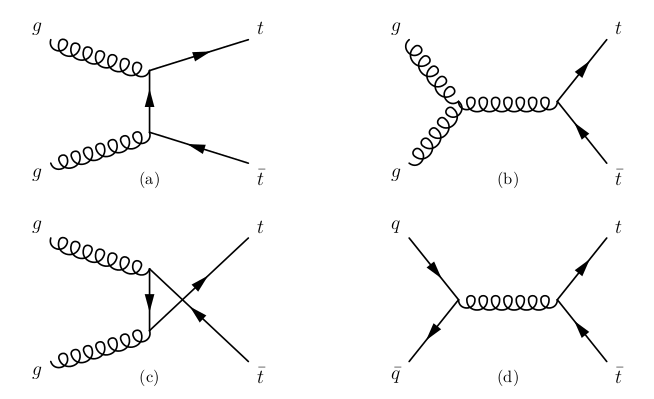
\includegraphics[width=\textwidth]{Figures/ttbarProductionLHC.png}
\caption{Lowest level diagrams for $t\bar{t}$ production at the LHC. Gluon scattering processes, {(a)}, {(b)}, and {(c)}, are the dominant processes at LHC energies, while quark scattering, process {(d)}, is the dominant one at TeVatron energies. \cite{SergeyThesis}}
\end{center}
\end{figure}

\begin{figure} \label{fig-singletopProductionLHC}
\begin{center}
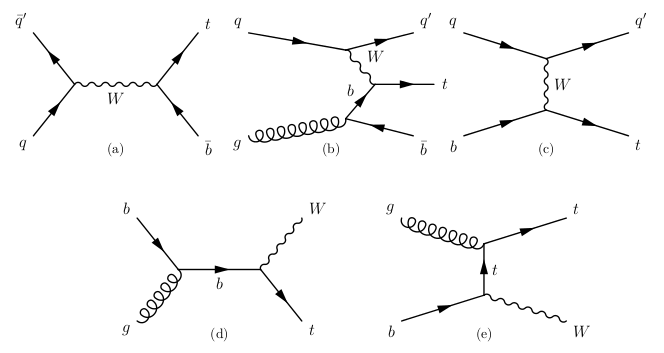
\includegraphics[width=\textwidth]{Figures/singletopProductionLHC.png}
\caption{Leading-order level diagrams for single top production at the LHC. {(a)} s-channel, {(b)} and {(c)} represent the t-channel, {(d)} and {(e)} both represent the two tW channels. \cite{SergeyThesis}}
\end{center}
\end{figure}

\begin{figure}
\begin{center}
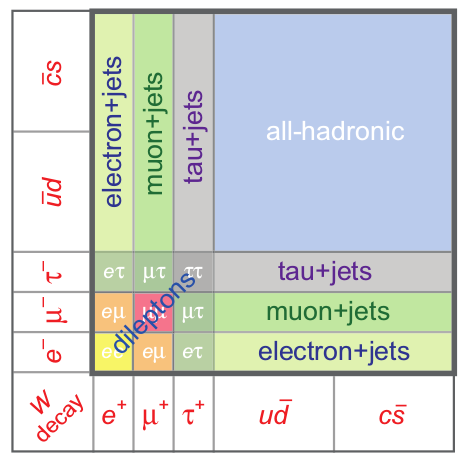
\includegraphics[width=0.5\textwidth]{Figures/ttbarDecayFractions.png}
\caption{Branching fractions of the W decays within top quark pairs. \cite{ttbarDecayFractions}}
\end{center}
\end{figure}

\begin{figure} \label{fig-ttgammaFeynmanDiagram}
\begin{center}
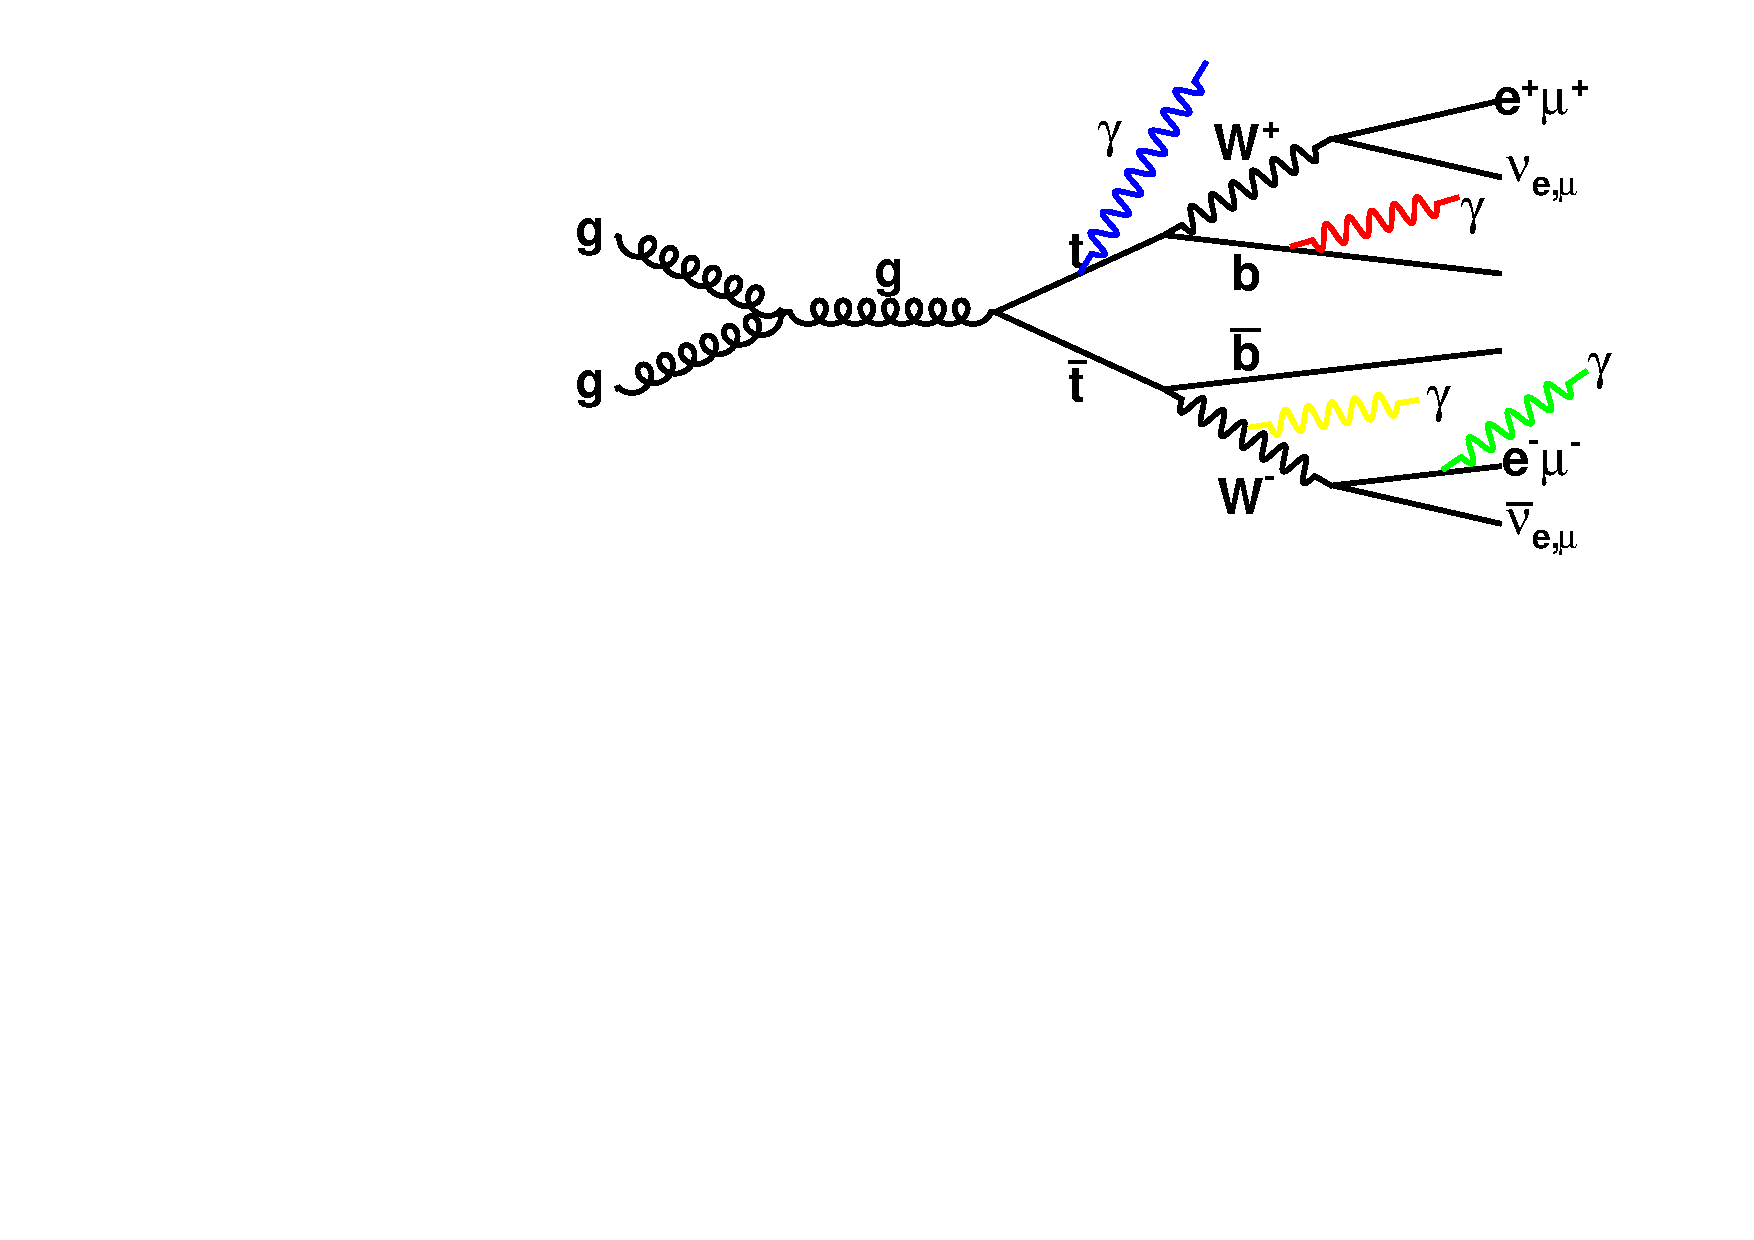
\includegraphics[width=0.9\textwidth]{Figures/ttgammaFeynmanDiagram.pdf}
\caption{}
\end{center}
\end{figure}